\section{Fisica della Materia e della Radiazione}
Si definisce \textbf{Materia Condensata} un insieme di particelle interagenti. In funzione del numero di particelle è possibile avere strutture differenti:
\begin{itemize}
	\item Nanostrutture $[\text{nm}]$ = caratterizzate da poche $(N<10^3)$ particelle interangeti Ovviamente essendoci pochi atomi si hanno sttrutture molto piccole;
	\item Mesostrutture $[\mu m]$ = caratterizate da un numero di particelle di $\sim  10^4$;
	\item Strutture macroscopiche $[mm]$ = sono caratterizzate da un $N_A$ di particelle interagenti.
\end{itemize}
Lo scopo del fisico è quello di costruire modelli fisici partendo dall'osservazione. L'osservazione di un determinato fenomeno conduce a porsi domande sulla sua natura prima, alle quali si cerca di rispondere attraverso la costruzione di un modello fisico-matematico che, se pur approssimato, segue i nostri schemi di comunicazione in modo oggettivo. Davanti a questa necessità nasce il problema di usare il modello pi\`u corretto. Gli interrogativi in questo caso sono nel discriminare quando utilizzare un modello classico e quando invece uno quantistico. La risposta non \`e assolutamente scontata e dipende da molte caratteristiche del sistema.
Le caratteristiche di un sistema sono in relazione anche alla \textit{finezza} con cui noi osserviamo il fenomeno. 

Se si conducono esperimenti su di un gas di elettroni, con i materiali che possiamo semplicemente trovare a casa nostra (fili di rame, resistenze, generatori, ecc..) le evidenze fenomenologiche che possiamo apprezzare sono tutte descrivibili con leggi classiche. Lo stesso gas di elettroni, raffreddato a temperature molto basse (vicine allo zero assoluto) e analizzato attraverso una tecnologia pi\`u raffinata, potrebbe mostrarci una fenomenologia in cui per far funzionare le leggi classiche usate precedentemente, sono necessarie approssimazioni, correzioni, teorie di campo medio, teorie efficaci, teorie fenomenologiche, quindi una serie di accorgimenti che suggeriscono all'indagatore che si ha a che fare con qualcosa di pi\`u profondo. Solitamente questo \textit{"qualcosa di pi\`u profondo"} trova una migliore spiegazione con una teoria quantistica, in particolar modo dall'introduzione naturale del parametro di scambio che governa molti sistemi quantistici e di cui non c\`e una diretta controparte classica.

Passando a cose pi\`u concrete, la descrizione di una particella, intesa come pacchetto d'onda, può cambiare molto in funzione al contesto in cui viene inserita. Se si ha sovrapposizione saranno presenti effetti quantistici che non si possono trascurare (per esempio l'interazione di scambio).
\subsection{Motivazioni storiche rilevanti}
In questo caso è necessario introdurre il discorso sulla diffrazione, riprendendo alcuni sviluppi storici della fisica di inizio '900. De Broglie, nella sua tesi di dottorato, postula la duplice natura della materia (corpuscolare ed ondulatoria) associando quindi, ad un certo momento $p$ una lunghezza d'onda $\lambda$. La relazione che unisce le due grandezze è la nota \textit{equazione di De Broglie}
\newl{\boxed{\lambda_D=\frac{h}{p}=\frac{h}{mv}. }}
Unendo il tutto con il momento angolare quantizzato di Bohr si ottiene la tanto interessante, quanto oscura, formula
\newl{\boxed{L = pr = n\frac{h}{\lambda} r  = n\frac{h}{2\pi r}r = n\frac{h}{2\pi} = n\hbar}}
che nasconde un mondo del tutto inesplorato. In primis, si nota subito la mancata definizione del mezzo oscillante. De Broglie infatti lascia aperta la questione del mezzo che viene perturbato e esce un momento angolare in funzione di multipli interi di $\hbar$, come se le orbite di Bohr fossero occupate da un'onda di lunghezza d'onda di De Broglie. La prima tappa del percorso conoscitivo della materia passa atraverso la verifica dell'ipotesi delle onde di De Broglie. A tal proposito, gli esperimenti di diffrazione di elettroni sono i più gettonati. In modo opportuno si preparano fasci di elettroni che vengono fatti diffrangere su di un cristallo. Uno schermo fluorescente (o un qualsiasi tipo di detector) è posto ad una certa distanza dal cristallo e raccoglie l'immagine diffratta. 
\begin{figure}
	\centering
	\fbox{
		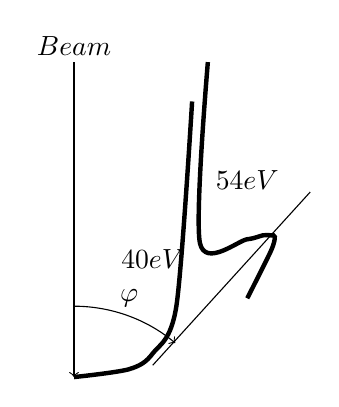
\begin{tikzpicture}[scale=1,auto=center]
			\draw [->] (0,4) -- (0,0) ;
			\node[] at (0,4.2)  {$Beam$};
			\node[] at (1,1.5) {$40eV$};
			\node[] at (2.2,2.5) {$54eV$};
			\node[] at (0.7,1) {$\varphi$};
			\draw [ultra thick] plot [smooth, tension=0.5] coordinates {(0,0) (0.7,0.1)  (1,0.3) (1.3, 0.9) (1.5,3.5) };
			\draw [ultra thick] plot [smooth, tension=0.5] coordinates {(2.2,1) (2.5,1.6) (2.55,1.78) (2.5,1.8) (2.4,1.8) (2.2,1.75) (1.6, 1.7) (1.7, 4)};
			\draw (1,0.15) -- (3,2.35);
			\draw[->] (0,0.9) arc (90:50:2);

		\end{tikzpicture}
	}
	\caption{Grafico dell'esperimento di Davisson-Germer. Viene plottata l'intensità degli elettroni scatterati contro l'angolo di scattering. Per $E=54eV$ si ha $\varphi=50^o$}
	\label{Davisson}
\end{figure}
Come si può notare in Fig.~\ref{Davisson}, per un'energia di $54eV$ si ha un picco di elettroni scatterati per $\phi=50^o$. Questo fenomeno lo si spiega solo pensando alla materia in modo ondulatorio, in quanto, per la legge di Bragg, avrò scattering solo quando all'energia del fascio corrisponderà una lunghezza d'onda comparabile con quella del size del reticolo, che nel caso di un solido sar\`a identificato dal passo del reticolo cristallino.
\subsection{Pacchetto d'onda}
Con la precedente premessa, il modo migliore per descrivere gli elettroni è attraverso  pacchetti d'onda non sovrapposti in cui $p\gg (\Delta p)$ e  $V/N \gg (\Delta r)^3$. In questo modo  è possibile usare un modello semi-classico rappresentato, come detto precedentemente, dalla lunghezza termica di De Broglie
\newl{\lambda_D=\frac{h}{p}=\frac{h}{\sqrt{2mE_C}} = \left(\frac{h^2}{3mK_BT}\right)^{\frac{1}{2}}}
con cui è possibile verificare che 
\newl{\frac{N}{V}\lambda_D^3 = \frac{N}{V}\left(\frac{h^2}{3mK_BT}\right)^{\frac{3}{2}}\ll 1.}
Si raggiunge la stessa conclusione partendo dal principio di indeterminazione di Heisenberg scritto nella ususale forma
\newl{\Delta r \cdot \Delta p \geq h.}
da cui è possibile ricavare
\newl{\frac{V}{N}p^3 \gg (\Delta r) \cdot (\Delta p) \geq h^3}
sapendo che $p=(3mK_BT)^{\frac{1}{2}}$ si ottiene nuovamente
\newl{\frac{N}{V}\left(\frac{h^2}{3mK_BT}\right)^{\frac{3}{2}}\ll 1.}
Un sistema può quindi essere modellizzato in modo classico per \textbf{densità} molto alte, \textbf{temperature} molto basse e \textbf{masse} molto piccole. Alcuni esempi sono dati da
\begin{itemize}
	\item Gas di idrogeno $[T\sim 0.26 K]$ sotto questa temperatura può essere modellizzato con le leggi classiche della cinetica dei gas;
	\item Elettroni di conduzione $[T \sim 1.8\cdot 10^5K]$ per modellizzare questo sistema è necessario usare modelli quantistici;
	\item Molti fotoni $(>10^3)$ si ha il campo elettromagnetico classico, quindi le equazioni di Maxwell;
	\item Pochi fotoni $(<10)$ si ha la QED (Quantum Elettro Dynamic).
\end{itemize}
